\section{Introduction}
\label{sec:intro}

\begin{figure}[ht]
    \centering
    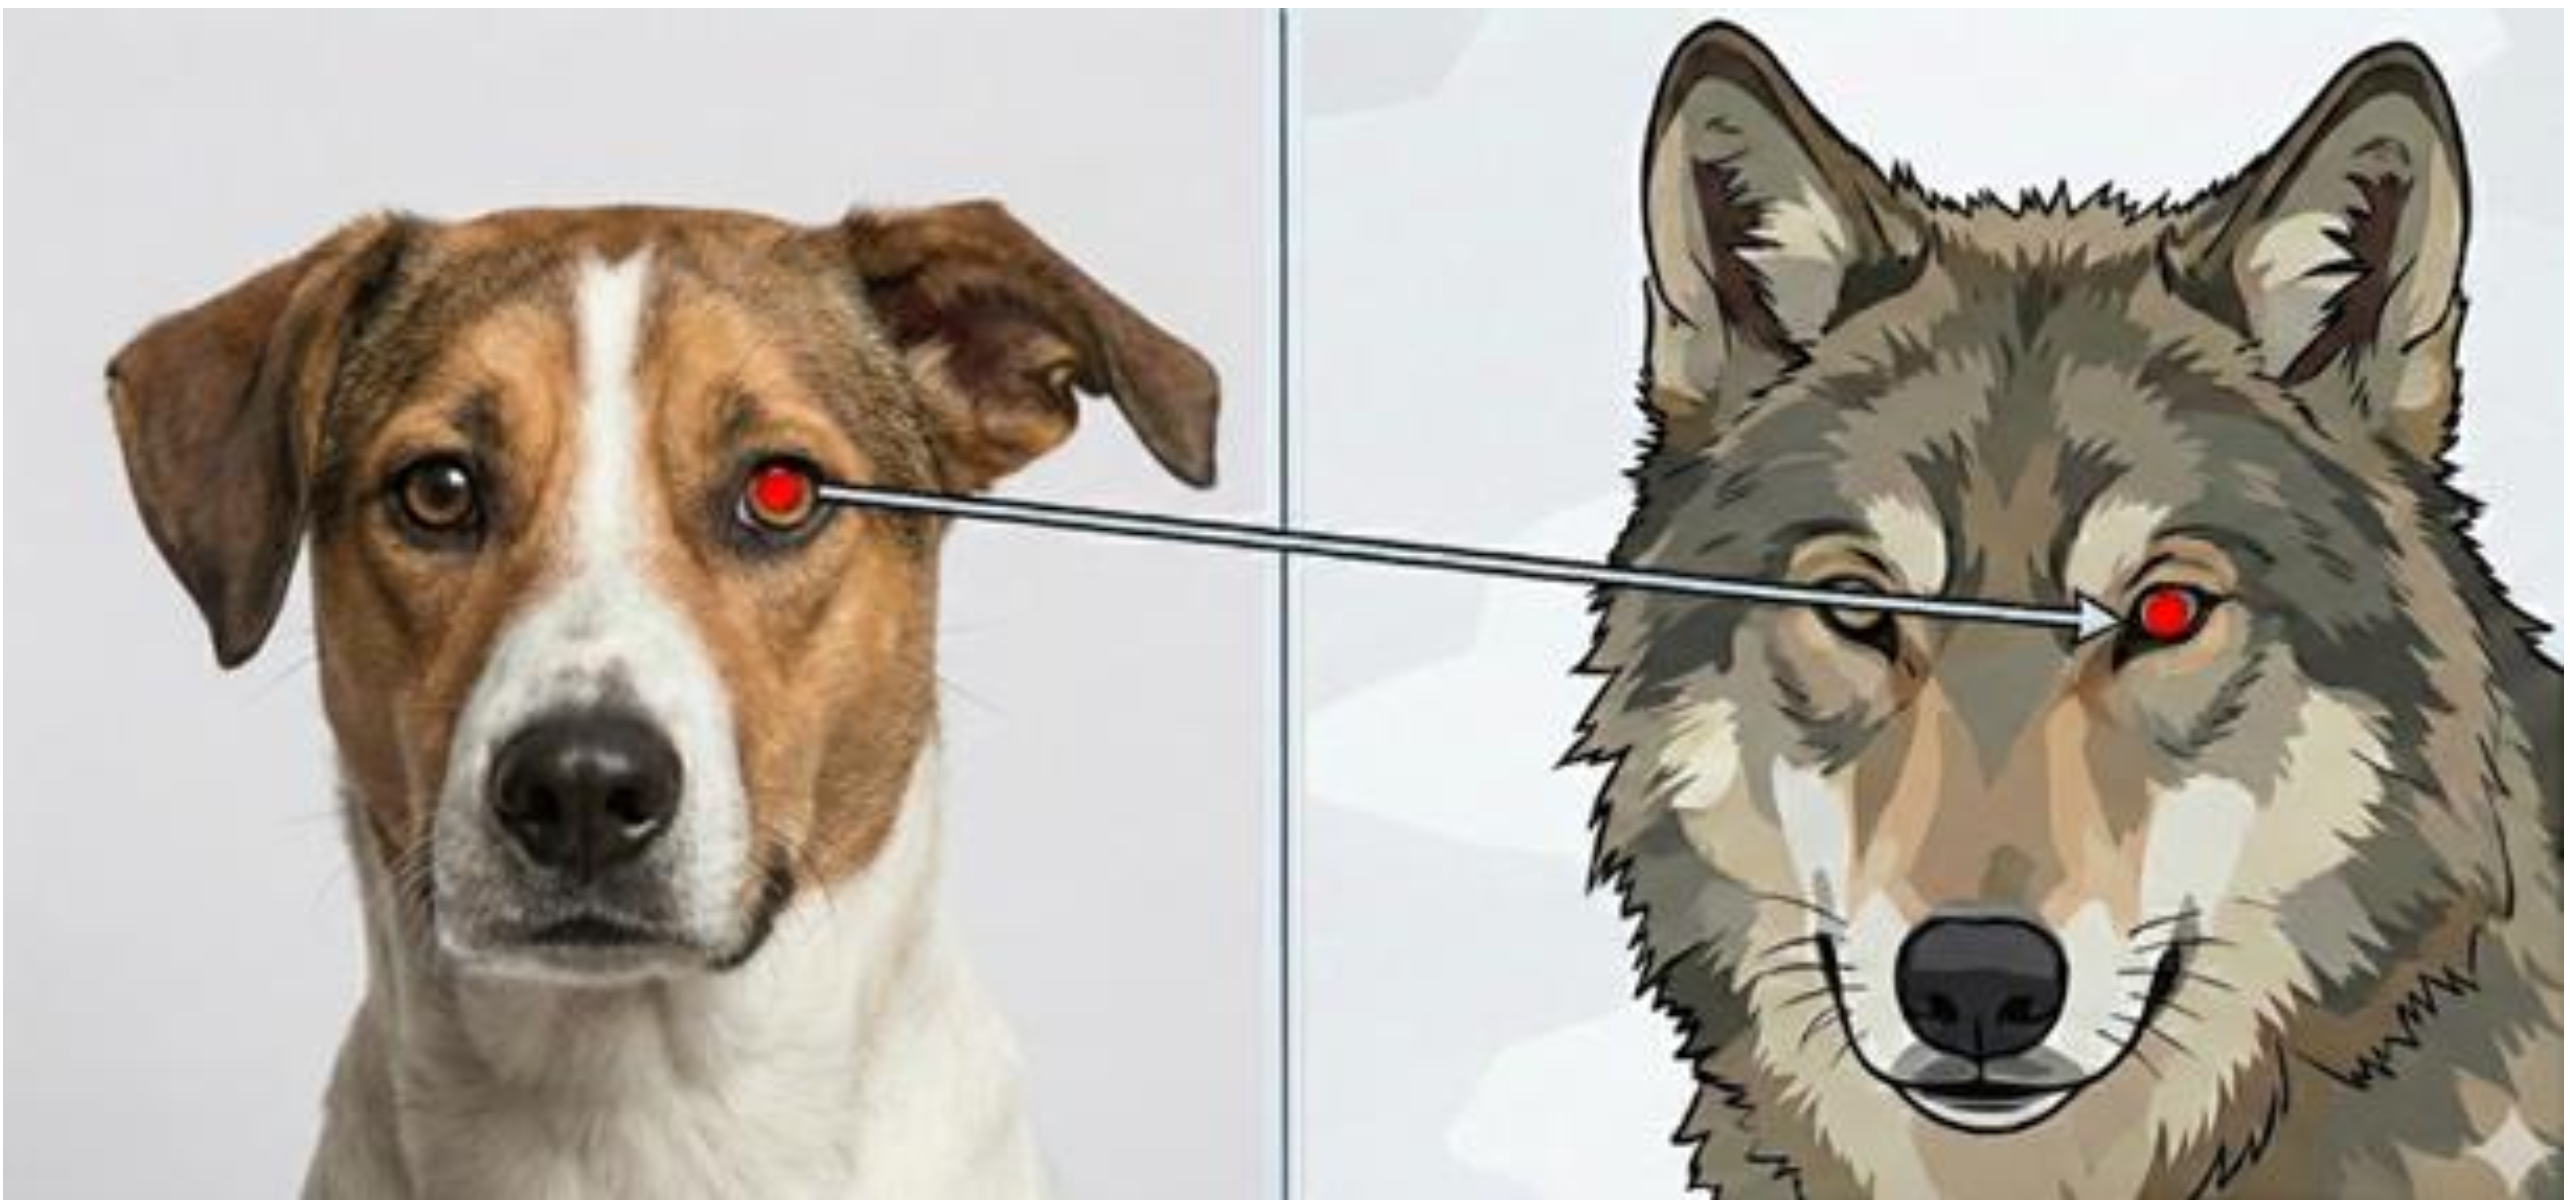
\includegraphics[width=\columnwidth]{img/teaser.png}
    \caption{Semantic correspondence across domains: matching the left eye of a dog in a photograph to the left eye of a wolf in an illustration.}
    \label{fig:teaser}
\end{figure}

Semantic correspondence is the complex task of finding pixel-level matches between semantically similar parts of objects across different images. Unlike standard geometric matching, which typically aligns different views of the exact same physical scene, semantic matching requires models to inherently understand object similarities despite drastic variations. Objects may appear in entirely different viewpoints, scales, or contexts, and the images themselves may originate from completely different visual domains, such as natural photographs versus artistic paintings. Furthermore, the system must accurately distinguish semantically similar but geometrically distinct parts, such as differentiating a left paw from a right paw.

Recent research demonstrates that large-scale Visual Foundation Models (VFMs) encompass rich internal representations that naturally support dense matching tasks. These representations emerge without explicit supervision, offering a highly effective starting point for semantic correspondence.

The primary goal of this project is to establish pixel-accurate semantic correspondences between a source image with annotated keypoints and a target image, leveraging features extracted from pre-trained visual encoders (DINOv2, DINOv3, and SAM). 

To systematically address and evaluate this task on the SPair-71k benchmark, the project is structured into four main stages:
\begin{itemize}
    \item \textbf{Training-Free Baseline:} Evaluating how well frozen features encode correspondence using cosine similarity and standard argmax.
    \item \textbf{Light Fine-Tuning:} Unfreezing and adapting the final layers of the backbone with keypoint supervision to enhance matching performance.
    \item \textbf{Prediction Refinement:} Replacing the discrete argmax operation with a Windowed Soft-Argmax to achieve sub-pixel accuracy and robustness against local noise.
    \item \textbf{Extension:} Exploring advanced strategies, specifically Parameter-Efficient Fine-Tuning via Low-Rank Adaptation (LoRA).
\end{itemize}